			\begin{question}{30}{reconnaissance de courbes}{2}{}
            Parmi les différentes représentations de la figure suivante, laquelle représente une évolution exponentielle?
            \begin{figure}
              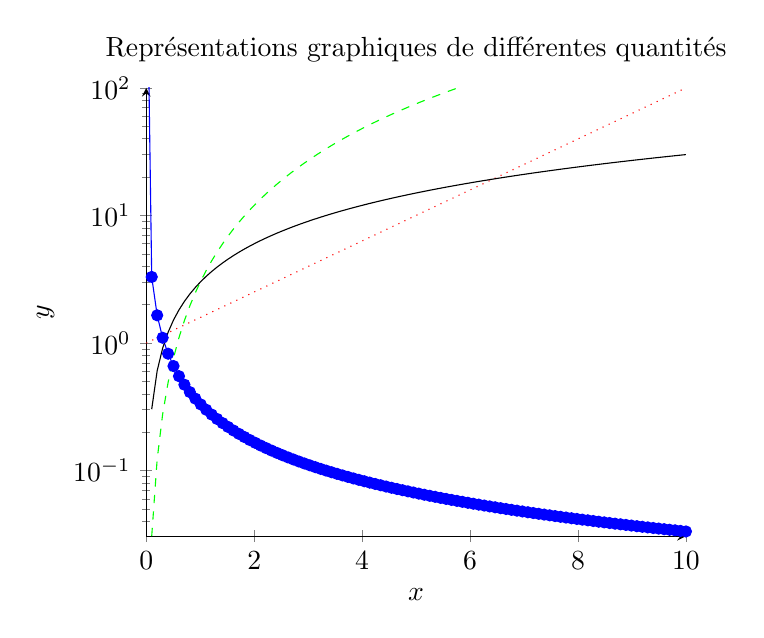
\begin{tikzpicture}
                  \begin{semilogyaxis}[
                        title = {Représentations graphiques de différentes quantités},
                        axis lines = left,
                        xlabel = $x$,
                        %minor x tick num = 4,
                        ylabel = $y$,
                        ymax=100,
                        /pgf/number format/.cd,%3 lignes dessous, utiliser spacers français au lieu d'anglais.
                        use comma,
                        1000 sep={\,}
                      ]
                      %Below the red curve
                      \addplot [
                        domain=0:10,
                        samples=100,
                        color=red,
                        style=dotted
                        %/pgf/text mark = {+}, %changer le marqueur text
                        %mark=o,
                      ]
                      {10^(0.2*x)};
                      \addplot [
                        domain=0.0001:10,
                        samples=100,
                        color=blue,
                        %/pgf/text mark = {+}, %changer le marqueur text
                        mark=*,
                      ]
                      {1/(3*x)};
                      \addplot [
                        domain=0:10,
                        samples=100,
                        color=black,
                        style=solid,
                        %/pgf/text mark = {+}, %changer le marqueur text
                        %mark=o,
                      ]
                      {3*x};
                      \addplot [
                        domain=0:10,
                        samples=100,
                        color=green,
                        style=dashed,
                        %/pgf/text mark = {+}, %changer le marqueur text
                        %mark=o,
                      ]
                      {3*x^2};
                  \end{semilogyaxis}
              \end{tikzpicture}
             \end{figure}
        \end{question}
        \begin{reponses}
            \item[false] La courbe bleue (cercles).
		    \item[true] La courbe rouge (pointillés).
		    \item[false] La courbe noire (pleine).
		    \item[false] La courbe verte (tirets).
		    \end{reponses}
        %%%%%%%%%%%%%%%%%%%%
         \begin{question}{N.A.}{reconnaissance de courbes}{1}{}
            Parmi les différentes représentations de la figure suivante, laquelle représente une évolution exponentielle?
            \begin{figure}
              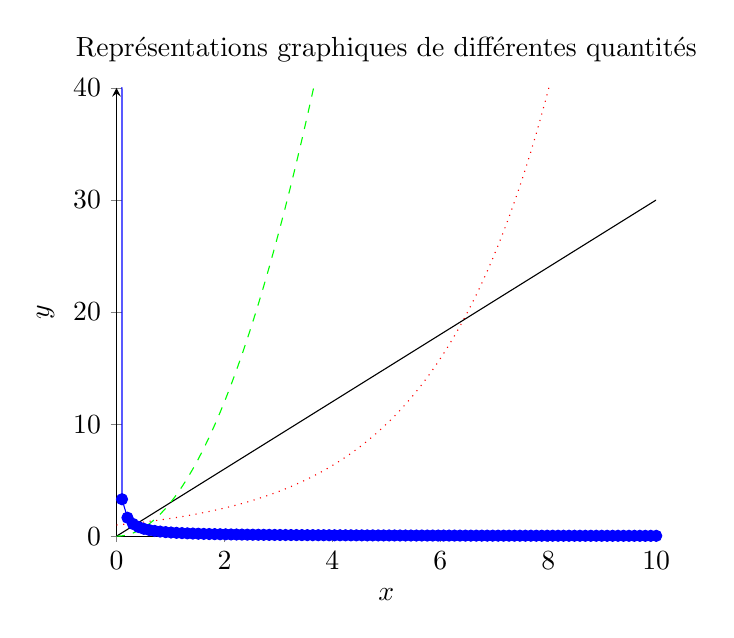
\begin{tikzpicture}
                  \begin{axis}[
                        title = {Représentations graphiques de différentes quantités},
                        axis lines = left,
                        xlabel = $x$,
                        %minor x tick num = 4,
                        ylabel = $y$,
                        ymin=0, ymax=40,
                        /pgf/number format/.cd,%3 lignes dessous, utiliser spacers français au lieu d'anglais.
                        use comma,
                        1000 sep={\,}
                      ]
                      %Below the red curve
                      \addplot [
                        domain=0:10,
                        samples=100,
                        color=red,
                        style=dotted
                        %/pgf/text mark = {+}, %changer le marqueur text
                        %mark=o,
                      ]
                      {10^(0.2*x)};
                      \addplot [
                        domain=0.0001:10,
                        samples=100,
                        color=blue,
                        mark=*,
                        %/pgf/text mark = {+}, %changer le marqueur text
                      ]
                      {1/(3*x)};
                      \addplot [
                        domain=0:10,
                        samples=100,
                        color=black,
                        %/pgf/text mark = {+}, %changer le marqueur text
                        %mark=o,
                        style=solid,
                      ]
                      {3*x};
                      \addplot [
                        domain=0:10,
                        samples=100,
                        color=green,
                        style=dashed,
                        %/pgf/text mark = {+}, %changer le marqueur text
                        %mark=o,
                      ]
                      {3*x^2};
                  \end{axis}
              \end{tikzpicture}
             \end{figure}
        \end{question}
        \begin{reponses}
            \item[false] La courbe bleue (cercles).
		    \item[true] La courbe rouge (pointillés).
		    \item[false] La courbe noire (pleine).
		    \item[false] La courbe verte (tirets).
		    \end{reponses}
        %%%%%%%%%%%%%%%%%%%%
        \begin{question}{NC}{reconnaissance de courbes}{2}{}
            Parmi les différentes courbes de la figure suivante, lesquelles représentent une évolution pseudo-périodique?
            \begin{figure}[!h]
              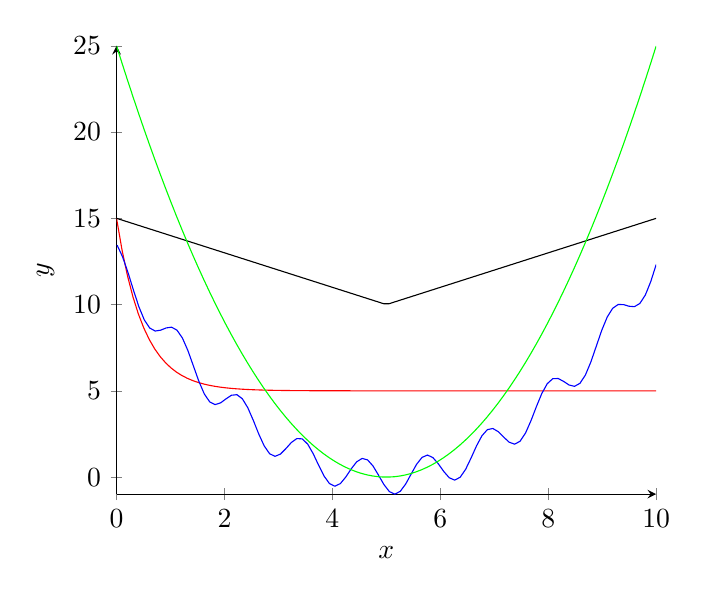
\begin{tikzpicture}
                  \begin{axis}[
                        title = { },
                        axis lines = left,
                        xlabel = $x$,
                        %minor x tick num = 4,
                        ylabel = $y$,
                        %ymin=0, ymax=40,
                        /pgf/number format/.cd,%3 lignes dessous, utiliser spacers français au lieu d'anglais.
                        use comma,
                        1000 sep={\,}
                      ]
                      %Below the red curve
                      \addplot [
                        domain=0:10,
                        samples=100,
                        color=red,
                        %/pgf/text mark = {+}, %changer le marqueur text
                        %mark=o,
                      ]
                      {10*exp(-2*x)+5};
                      \addplot [
                        domain=0.01:10,
                        samples=100,
                        color=blue,
                        %/pgf/text mark = {+}, %changer le marqueur text
                        %mark=o,
                      ]
                      {cos(2*3.14*50*x)+0.5*(x-5)^2};
                      \addplot [
                        domain=0:10,
                        samples=100,
                        color=black,
                        %/pgf/text mark = {+}, %changer le marqueur text
                        %mark=o,
                      ]
                      {abs(x-5)+10};
                      \addplot [
                        domain=0:10,
                        samples=100,
                        color=green,
                        %/pgf/text mark = {+}, %changer le marqueur text
                        %mark=o,
                      ]
                      {(x-5)^2};
                  \end{axis}
              \end{tikzpicture}
              \end{figure}
        \end{question}
        \begin{reponses}
            	\item[false]  La courbe noire
            	\item[false]   La courbe rouge
                \item[false]  La courbe verte
                \item[true]   La courbe bleue
            \end{reponses}
           %%%%%%%%%%%%%%%%%%%%%%%%%%%%%%%%%%%%%%%%%%%%%%%%%
              \begin{question}{N.A.}{reconnaissance de courbes}{2}{}
            Parmi les différentes représentations de la figure suivante, laquelle représente une évolution exponentielle?
            \begin{figure}
              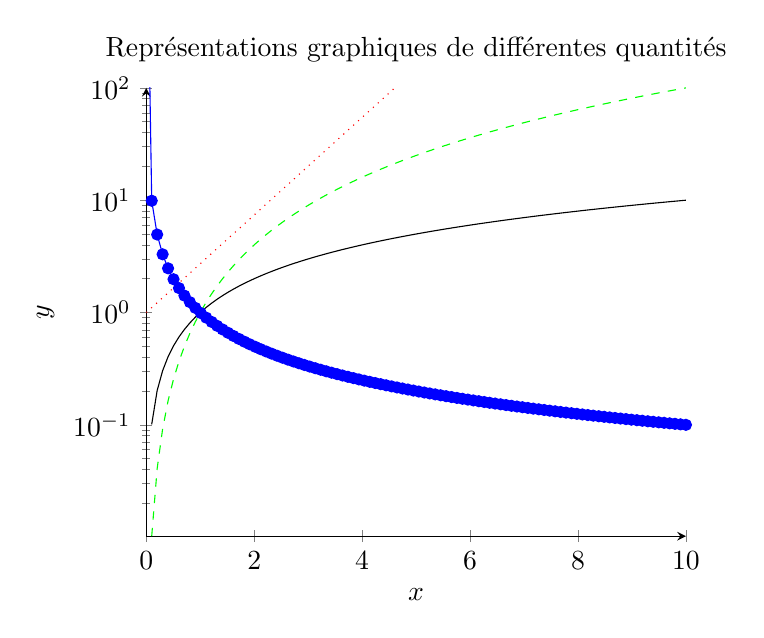
\begin{tikzpicture}
                  \begin{semilogyaxis}[
                        title = {Représentations graphiques de différentes quantités},
                        axis lines = left,
                        xlabel = $x$,
                        %minor x tick num = 4,
                        ylabel = $y$,
                        ymax=100,
                        /pgf/number format/.cd,%3 lignes dessous, utiliser spacers français au lieu d'anglais.
                        use comma,
                        1000 sep={\,}
                      ]
                      %Below the red curve
                      \addplot [
                        domain=0:10,
                        samples=100,
                        color=red,
                        style=dotted
                        %/pgf/text mark = {+}, %changer le marqueur text
                        %mark=o,
                      ]
                      {exp(x)};
                      \addplot [
                        domain=0.0001:10,
                        samples=100,
                        color=blue,
                        %/pgf/text mark = {+}, %changer le marqueur text
                        mark=*,
                      ]
                      {1/x};
                      \addplot [
                        domain=0:10,
                        samples=100,
                        color=black,
                        style=solid,
                        %/pgf/text mark = {+}, %changer le marqueur text
                        %mark=o,
                      ]
                      {x};
                      \addplot [
                        domain=0:10,
                        samples=100,
                        color=green,
                        style=dashed,
                        %/pgf/text mark = {+}, %changer le marqueur text
                        %mark=o,
                      ]
                      {x^2};
                  \end{semilogyaxis}
              \end{tikzpicture}
             \end{figure}
        \end{question}
        \begin{reponses}
            \item[false] La courbe bleue (cercles).
		    \item[true] La courbe rouge (pointillés).
		    \item[false] La courbe noire (pleine).
		    \item[false] La courbe verte (tirets).
		    \end{reponses}
        %%%%%%%%%%%%%%%%%%%%
        \begin{question}{N.A.}{reconnaissance de courbes}{2}{}
            Parmi les différentes représentations de la figure suivante, laquelle représente une évolution linéaire?
            \begin{figure}
              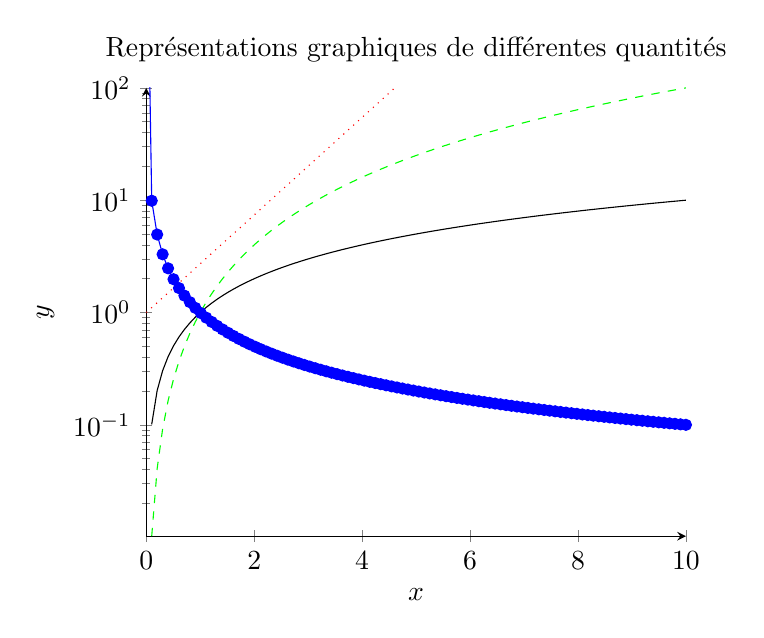
\begin{tikzpicture}
                  \begin{semilogyaxis}[
                        title = {Représentations graphiques de différentes quantités},
                        axis lines = left,
                        xlabel = $x$,
                        %minor x tick num = 4,
                        ylabel = $y$,
                        ymax=100,
                        /pgf/number format/.cd,%3 lignes dessous, utiliser spacers français au lieu d'anglais.
                        use comma,
                        1000 sep={\,}
                      ]
                      %Below the red curve
                      \addplot [
                        domain=0:10,
                        samples=100,
                        color=red,
                        style=dotted
                        %/pgf/text mark = {+}, %changer le marqueur text
                        %mark=o,
                      ]
                      {exp(x)};
                      \addplot [
                        domain=0.0001:10,
                        samples=100,
                        color=blue,
                        %/pgf/text mark = {+}, %changer le marqueur text
                        mark=*,
                      ]
                      {1/x};
                      \addplot [
                        domain=0:10,
                        samples=100,
                        color=black,
                        style=solid,
                        %/pgf/text mark = {+}, %changer le marqueur text
                        %mark=o,
                      ]
                      {x};
                      \addplot [
                        domain=0:10,
                        samples=100,
                        color=green,
                        style=dashed,
                        %/pgf/text mark = {+}, %changer le marqueur text
                        %mark=o,
                      ]
                      {x^2};
                  \end{semilogyaxis}
              \end{tikzpicture}
             \end{figure}
        \end{question}
        \begin{reponses}
            \item[false] La courbe bleue (cercles).
		    \item[false] La courbe rouge (pointillés).
		    \item[true] La courbe noire (pleine).
		    \item[false] La courbe verte (tirets).
		    \end{reponses}
        %%%%%%%%%%%%%%%%%%%%
        \begin{question}{N.A.}{reconnaissance de courbes}{3}{}
            On étudie l'évolution d'une population de bactérie au cours du temps. Soit N(t) le nombre de bactéries observées au temps t. N(t) est défini par la loi d'évolution suivante :$N_{cellules}=\frac{1000}{1+2exp(-2(t-3))}$. Parmi les différentes représentations de la figure suivante, laquelle représente l'évolution de N(t)?            
            \begin{figure}
              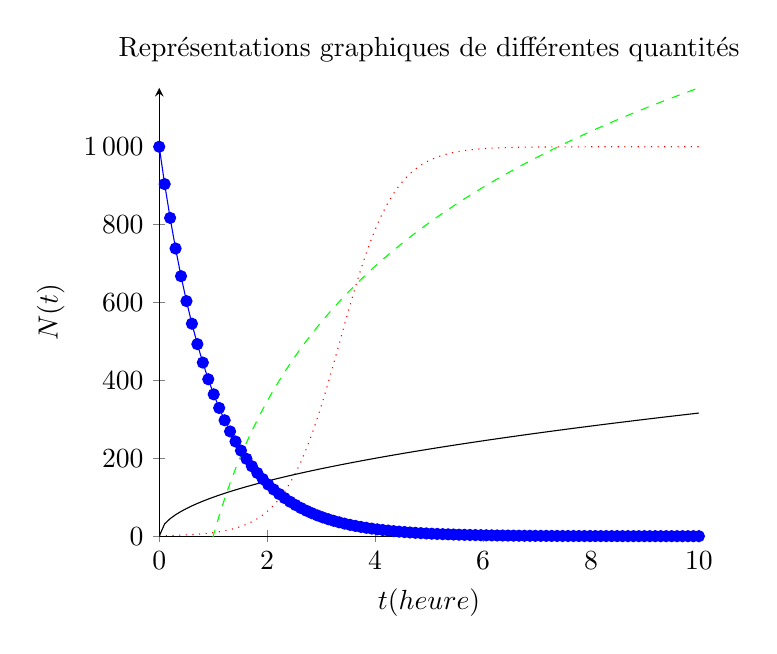
\begin{tikzpicture}
                  \begin{axis}[
                        title = {Représentations graphiques de différentes quantités},
                        axis lines = left,
                        xlabel = $t (heure)$,
                        %minor x tick num = 4,
                        ylabel = $N(t)$,
                        ymin=0,
                        /pgf/number format/.cd,%3 lignes dessous, utiliser spacers français au lieu d'anglais.
                        use comma,
                        1000 sep={\,}
                      ]
                      %Below the red curve
                      \addplot [
                        domain=0:10,
                        samples=100,
                        color=red,
                        style=dotted
                        %/pgf/text mark = {+}, %changer le marqueur text
                        %mark=o,
                      ]
			          {1000/(1+2*exp(-2*(x-3)))};
                      \addplot [
                        domain=0:10,
                        samples=100,
                        color=blue,
                        %/pgf/text mark = {+}, %changer le marqueur text
                        mark=*,
                      ]
                      {1000*exp(-x)};
                      \addplot [
                        domain=0:10,
                        samples=100,
                        color=black,
                        style=solid,
                        %/pgf/text mark = {+}, %changer le marqueur text
                        %mark=o,
                      ]
                      {100*sqrt(x)};
                      \addplot [
                        domain=0:10,
                        samples=100,
                        color=green,
                        style=dashed,
                        %/pgf/text mark = {+}, %changer le marqueur text
                        %mark=o,
                      ]
                      {500*ln(x)};
                  \end{axis}
              \end{tikzpicture}
             \end{figure}
        \end{question}
        \begin{reponses}
            \item[false] La courbe bleue (cercles).
		    \item[true] La courbe rouge (pointillés).
		    \item[false] La courbe noire (pleine).
		    \item[false] La courbe verte (tirets).
		    \end{reponses}
        %%%%%%%%%%%%%%%%%%%%
            \begin{question}{30}{Fonctions usuelles}{2}{/}
            On étudie l'évolution d'une population de bactérie au cours du temps. Soit N(t) le nombre de bactéries observées au temps t. N(t) est défini par la loi d'évolution suivante : $N(t) = 10\exp{-2t}$. Parmi les différentes représentations de la figure suivante, laquelle représente l'évolution de N(t)?            \begin{figure}
              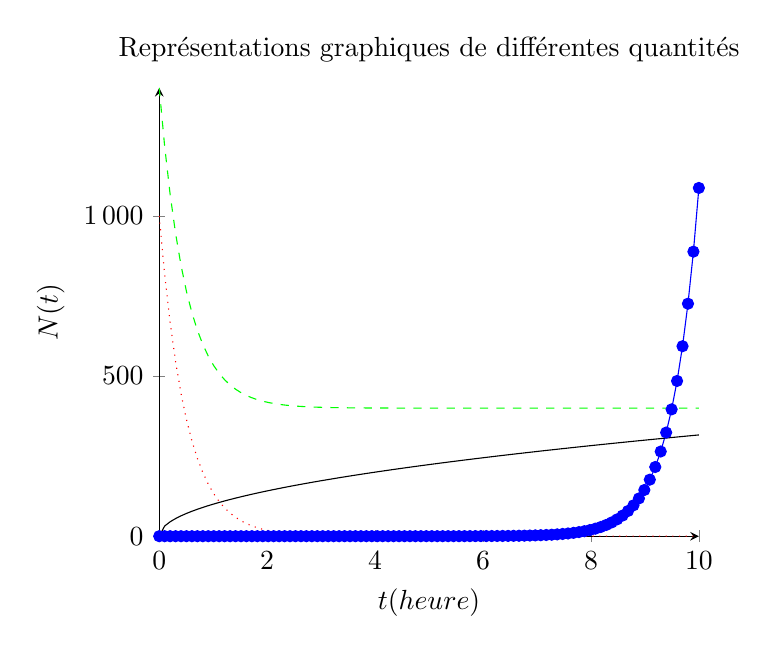
\begin{tikzpicture}
                  \begin{axis}[
                        title = {Représentations graphiques de différentes quantités},
                        axis lines = left,
                        xlabel = $t (heure)$,
                        %minor x tick num = 4,
                        ylabel = $N(t)$,
                        %ymax=100,
                        /pgf/number format/.cd,%3 lignes dessous, utiliser spacers français au lieu d'anglais.
                        use comma,
                        1000 sep={\,}
                      ]
                      %Below the red curve
                      \addplot [
                        domain=0:10,
                        samples=100,
                        color=red,
                        style=dotted
                        %/pgf/text mark = {+}, %changer le marqueur text
                        %mark=o,
                      ]
                      {1000*exp(-2*x)};
                      \addplot [
                        domain=0:10,
                        samples=100,
                        color=blue,
                        %/pgf/text mark = {+}, %changer le marqueur text
                        mark=*,
                      ]
                      {1e-3*exp(2*x-5)/3};
                      \addplot [
                        domain=0:10,
                        samples=100,
                        color=black,
                        style=solid,
                        %/pgf/text mark = {+}, %changer le marqueur text
                        %mark=o,
                      ]
                      {sqrt(x)*100};
                      \addplot [
                        domain=0:10,
                        samples=100,
                        color=green,
                        style=dashed,
                        %/pgf/text mark = {+}, %changer le marqueur text
                        %mark=o,
                      ]
                      {1000*exp(-2*x)+400};
                  \end{axis}
              \end{tikzpicture}
             \end{figure}
        \end{question}
        \begin{reponses}
            \item[false] La courbe bleue (cercles).
		    \item[true] La courbe rouge (pointillés).
		    \item[false] La courbe noire (pleine).
		    \item[false] La courbe verte (tirets).
		    \end{reponses}
        %%%%%%%%%%%%%%%%%%%%
